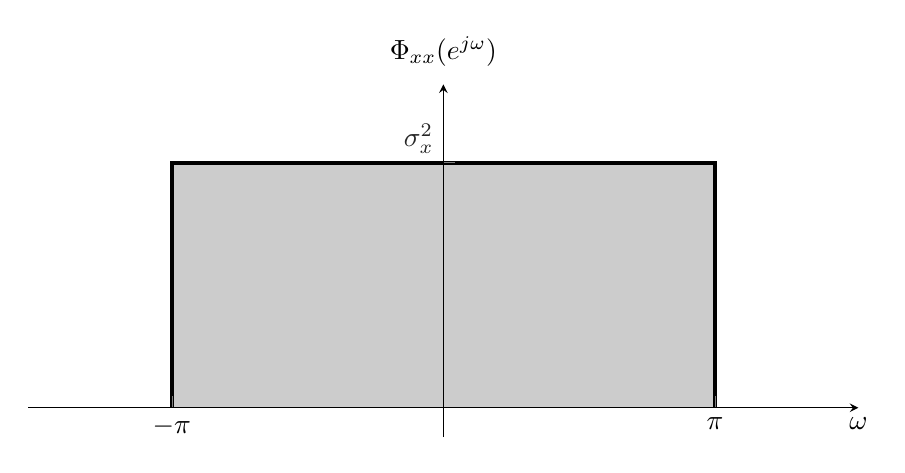
\begin{tikzpicture} 
\begin{axis}[
axis lines*=middle,
enlargelimits = true,
xmax=4,
xmin=-4,
ymin=0,
ymax=1.2,
width=\textwidth,
height=0.5\textwidth,
axis line style={->,>=stealth},
xlabel={$\omega$},
ylabel={$\Phi_{xx}(e^{j\omega})$},
yticklabel style = {yshift=0.3cm},
every axis x label/.style={
    at={(ticklabel* cs:1)},
    anchor=north,
},
every axis y label/.style={
    at={(ticklabel* cs:1)},
    anchor=south,
    yshift=0.1cm,
},
xtick=\empty,
ytick={1},
xtick={-3.14, 3.14},
xticklabels={$-\pi$, $\pi$},
yticklabels={$\sigma_x^2$},
%xmajorgrids,
%ymajorgrids,
axis on top,
every outer y axis line/.append style={white!15!black},
every y tick label/.append style={font=\color{white!15!black}},
legend style={draw=white!15!black,fill=white,legend cell align=left}]
\addplot[domain=-3.14:3.14, samples=2,line width=1.5pt,fill=black!20] coordinates {(-3.14, 0) (-3.14, 1) (3.14, 1) (3.14, 0)};
\end{axis}
\end{tikzpicture}
